\section{Deep and shallow semantic construction}
\label{sec:motivation}

Consider the
following (toy) sentence:
\begin{examples}
\label{ex:cat}
  \item Every fat cat chased some dog.
\end{examples}
It exhibits several kinds of ambiguity, including a quantifier scope
ambiguity and lexical
ambiguities---e.g., the nouns ``cat'' and ``dog'' have 8 and 7
WordNet senses respectively.  Simplifying slightly by ignoring tense
information, two of its readings are shown as logical forms below;
these can be represented as trees as shown in Fig.~\ref{fig:1}.
%  (but see Section~\ref{sec:extensions})

\begin{examples}
\item $\sem{\_every\_q\_1}(x, \sem{\_fat\_j\_1}(e',x) \wedge
    \sem{\_cat\_n\_1}(x),$\\
\hspace*{0.1in} $\sem{\_some\_q\_1}(y, \sem{\_dog\_n\_1}(y),$\\
\hspace*{0.2in}$\sem{\_chase\_v\_1}(e,x,y)))$
\label{ex:fat-cat-1}
\item $\sem{\_some\_q\_1}(y, \sem{\_dog\_n\_2}(y),$\\
\hspace*{0.1in}$\sem{\_every\_q\_1}(x, \sem{\_fat\_j\_1}(e',x) \wedge
    \sem{\_cat\_n\_2}(x), $\\
\hspace*{0.2in}$\sem{\_chase\_v\_1}(e,x,y)))$
\label{ex:fat-cat-2}
\end{examples}


\begin{figure}[t]
\centering
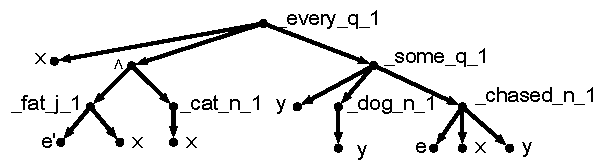
\includegraphics[scale=0.8]{pic-cat-chased-dog} \\
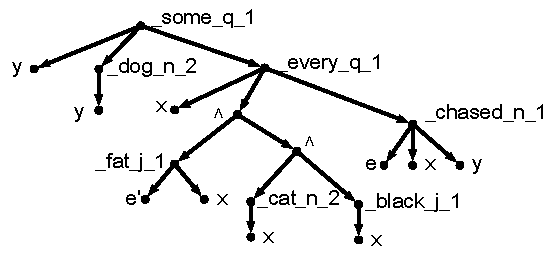
\includegraphics[scale=0.8]{pic-cat-chased-dog-2}
\caption{Semantic representations (\ref{ex:fat-cat-1}) and
  (\ref{ex:fat-cat-2}) as trees. \label{fig:1}}
\end{figure}


Now imagine trying to extract semantic information from the output of
a part-of-speech ({\sc pos}) tagger by using the word lemmas as
lexical predicate symbols.  Such a semantic representation is highly
partial.  It will use predicate symbols such as $\sempred{\_cat\_n}$,
which might resolve to the predicate symbols $\sem{\_cat\_n\_1}$ or
$\sem{\_cat\_n\_2}$ in the complete semantic representation.  (Notice
the different fonts for the ambiguous and unambiguous predicate
symbols.)  But most underspecification formalisms (e.g., {\sc mrs}
\cite{copestake:etal:2005} and {\sc clls} \cite{egg:etal:2001}) are
unable to represent semantic information that is as partial as what we
get from a {\sc pos} tagger because they cannot underspecify
predicate-argument structure.  \rmrs\ \cite{copestake:2007a} is 
designed to address this problem.  In \rmrs, the
information we get from the {\sc pos} tagger is as follows:

\begin{examples}
\item \label{ex:cat-pos}
$l_1:a_1:\sempred{\_every\_q}(x_1)$, \\
$l_{41}:a_{41}:\sempred{\_fat\_j}(e')$,\\
$l_{42}:a_{42}:\sempred{\_cat\_n}(x_3)$\\
$l_5:a_5:\sempred{\_chase\_v}(e)$, \\
$l_6:a_6:\sempred{\_some\_q}(x_6)$, \\
$l_9:a_9:\sempred{\_dog\_n}(x_7)$
\end{examples}

This \rmrs\ expresses only that certain predications are present in
the semantic representation---it doesn't say anything about
semantic scope, about most arguments of the
predicates (e.g., $\sempred{\_chase\_v}(e)$ doesn't say who chases
whom), or about the coindexation of variables ($\sempred{\_every\_q}$
binds the variable $x_1$, whereas $\sempred{\_cat\_n}$ speaks about
$x_3$), and it maintains the lexical ambiguities.  Technically, it
consists of six \emph{elementary predications} ({\sc ep}s), one for
each word lemma in the sentence; each of them is prefixed by a
\emph{label} and an \emph{anchor}, which are essentially variables
that refer to nodes in the trees in Fig.~\ref{fig:1}.  We can say that
the two trees \emph{satisfy} this \rmrs\ because it is possible to map
the labels and anchors in (\ref{ex:cat-pos}) into nodes in each tree
and variable names like 
$x_1$ and $x_3$ into variable names in the tree in such a way that the
predications of the nodes that labels and anchors denote are 
consistent with those in the {\sc ep}s of (\ref{ex:cat-pos})---e.g.,
$l_1$ and $a_1$
can map to the root of the first tree in Fig.~\ref{fig:1}, $x_1$ to
$x$, and the root label 
$\sem{\_every\_q\_1}$ is consistent with the {\sc ep} predicate
$\sempred{\_every\_q}$.

% The lack of semantic dependencies rendered by a {\sc pos} tagger means
% we have unique arguments to each predicate symbol (e.g., see $x_1$ and
% $x_3$ in (\ref{ex:cat-pos}), compared with the {\em same} variable $x$
% in the semantic representations (\ref{ex:fat-cat-1}) and
% (\ref{ex:fat-cat-2})).

There are of course many other trees (and thus, fully specific
semantic representations such as (\ref{ex:fat-cat-1})) that are
described equally well by the \rmrs\ (\ref{ex:cat-pos}); this is not
surprising, given that the semantic output from the {\sc
  pos} tagger is so incomplete.  If we have
information about subjects and objects from a chunk parser
like Cass \cite{abney:1996}, we can represent it in a more detailed
\rmrs:

\begin{examples}
\item 
$l_1:a_1:\sempred{\_every\_q}(x_1)$, \\
$l_{41}:a_{41}:\sempred{\_fat\_j}(e')$,\\
$l_{42}:a_{42}:\sempred{\_cat\_n}(x_3)$\\
$l_5:a_5:\sempred{\_chase\_v}(e)$, \\
\hspace*{0.1in} $\ARG_1(a_5,x_4),
\ARG_2(a_5,x_5)$\\ 
$l_6:a_6:\sempred{\_some\_q}(x_6)$, \\
$l_9:a_9:\sempred{\_dog\_n}(x_7)$\\
$x_3=x_4$, $x_5=x_7$
\label{ex:cat-partial-parser}
\end{examples}

This introduces two new types of atoms.   $x_3=x_4$
means that $x_3$ and $x_4$ map to the same
variable in any fully specific logical form; e.g., both to the
variable $x$ in Fig.~\ref{fig:1}.   $\ARG_i(a,z)$ (and
$\ARG_i(a,h)$) express that the $i$-th child (counting from 0) of the
node to which the anchor $a$ refers is the variable name that $z$
denotes (or the node that the {\em hole} $h$ denotes).  So unlike
earlier underspecification formalisms, \rmrs\ can specify the
predicate of an atom separately from its
arguments; this is necessary for supporting parsers where information
about lexical subcategorisation is absent. If we also allow atoms of
the form $\ARG_{\{2,3\}}(a,x)$ to express uncertainty as to whether
$x$ is the second or third child of the anchor $a$, then \rmrs\ can
even specify the arguments to a predicate while underspecifying their
position.  This is useful for specifying arguments to \_give\_v when a
parser doesn't handle unbounded dependencies and is faced with
{\em Which bone did you give the dog?} vs.\ {\em To which dog did you
  give the bone?}

Finally, the \rmrs\ (\ref{ex:cat-erg}) is a notational variant of the
{\sc mrs} derived by the {\sc erg}, a wide-coverage deep grammar:
\begin{examples}
\item $l_1:a_1\handel\sempred{\_every\_q\_1}(x_1),$\\
\hspace*{0.1in}$\mathsf{RSTR}(a_1,h_2),
\mathsf{BODY}(a_1,h_3)$\\ 
$l_{41}:a_{41}\handel\sempred{\_fat\_j\_1}(e'), \ARG_1(a_{41},x_2)$\\
$l_{42}:a_{42}\handel\sempred{\_cat\_n\_1}(x_3)$\\
$l_5:a_5\handel\sempred{\_chase\_v\_1}(e)$,\\
\hspace*{0.1in}$\ARG_1(a_5,x_4),
\ARG_2(a_5,x_5)$\\ 
$l_6:a_6\handel\sempred{\_some\_q\_1}(x_6)$,\\
\hspace*{0.1in}$\mathsf{RSTR}(a_6,h_7),
\mathsf{BODY}(a_6,h_8)$\\ 
$l_9:a_9\handel\sempred{\_dog\_n\_1}(x_7)$\\
$h_2=_q l_{42}, l_{41}=l_{42}, h_7 =_q l_9$\\
$x_1=x_2, x_2=x_3, x_3=x_4,$\\
$x_5=x_6, x_5=x_7$
\label{ex:cat-erg}
\end{examples}

$\mathsf{RSTR}$ and $\mathsf{BODY}$ are conventional names
for the $\ARG_1$ and $\ARG_2$ of a quantifier predicate symbol.  Atoms
like $h_2 \qeq l_{42}$ (``qeq'') specify a certain kind of
``outscopes'' relationship between the hole and the label, and are
used here to underspecify the scope of the two quantifiers.
Notice that the labels of the {\sc ep}s for ``fat'' and ``cat'' are
stipulated to be equal in (\ref{ex:cat-erg}), whereas the anchors are not.  In
the tree, it is the anchors that are mapped to the nodes with the
labels $\sem{\_fat\_j\_1}$ and $\sem{\_cat\_n\_1}$; the label is
mapped to the conjunction node just above them.  In other words, the
role of the anchor in an {\sc ep} is to connect a predicate to its
arguments, while the role of the label is to connect the {\sc ep} to
the surrounding formula.  Representing conjunction with label sharing
stems from \mrs\ and provides compact representations.

Finally, (\ref{ex:cat-erg}) uses predicate symbols like
$\sempred{\_dog\_n\_1}$ that are meant to be more specific than 
symbols like $\sempred{\_dog\_n}$ which the earlier \rmrs s used.
This reflects the fact that the deep grammar performs some lexical
disambiguation that the chunker and {\sc pos} tagger don't.  The fact
that the former symbol should be more specific than the latter can be
represented using SPEC atoms like $\sempred{\_dog\_n\_1}\sqsubseteq
\sempred{\_dog\_n}$.
Note that even a deep grammar will not fully disambiguate to
semantic predicate symbols, such as WordNet senses, and so
$\sempred{\_dog\_n\_1}$ can still be consistent with multiple symbols
like $\sem{\_dog\_n\_1}$ and $\sem{\_dog\_n\_2}$ in the semantic
representation.  However, unlike the output of a
{\sc pos} tagger, an \rmrs\ symbol that's output by a deep grammar is
consistent 
with symbols that all have the {\em same} arity, because a deep grammar
fully determines lexical subcategorisation.

In summary, \rmrs\ allows us to represent in a uniform way
the (partial) semantics
that can be extracted from a wide range of {\sc nlp} tools.
This is useful for hybrid systems which exploit shallower
analyses when deeper parsing fails, or which try to match
deeply parsed queries against shallow parses of large corpora;
and in fact, \rmrs\ is gaining popularity as a practical interchange
format for exactly these purposes \cite{copestake:2003}.
However, \rmrs\ is still relatively ad-hoc in that its
formal semantics is
not defined; we don't know, formally, what an \rmrs\ \emph{means} in
terms of semantic representations like (\ref{ex:fat-cat-1}) and
(\ref{ex:fat-cat-2}), and this hinders our ability to design efficient
algorithms for processing \rmrs. The purpose of this paper is to lay
the groundwork for fixing this problem.

%%% Local Variables: 
%%% mode: latex
%%% TeX-master: "rmrs-08"
%%% End: 
